\section{Date: 2026-11-25}
\noindent \textbf{Series ID: DGS1MO} 

\noindent This series is titled Market Yield on U.S. Treasury Securities at 1-Month Constant Maturity, Quoted on an Investment Basis and has a frequency of Daily. The units are Percent and the seasonal adjustment is Not Seasonally Adjusted.The observation start date is 2001-07-31 and the observation end date is 2026-11-23.The popularity of this series is 76. \\ 

\noindent \textbf{Series ID: DPRIME} 

\noindent This series is titled Bank Prime Loan Rate and has a frequency of Daily. The units are Percent and the seasonal adjustment is Not Seasonally Adjusted.The observation start date is 1955-08-04 and the observation end date is 2026-11-23.The popularity of this series is 76. \\ 

\subsection{Raw Regression}
\noindent Regresses the two series against each other directly. A significant result here can come just as easily from both series sharing a long-run trend as from any real relationship.

\begin{center}
\begin{tabular}{lclc}
\toprule
\textbf{Dep. Variable:}      & value\_fred\_DPRIME & \textbf{  R-squared:         } &     0.982   \\
\textbf{Model:}              &         OLS         & \textbf{  Adj. R-squared:    } &     0.982   \\
\textbf{Method:}             &    Least Squares    & \textbf{  F-statistic:       } & 3.368e+05   \\
\textbf{Date:}               &   Wed, 25 Nov 2026  & \textbf{  Prob (F-statistic):} &     0.00    \\
\textbf{Time:}               &       20:47:06      & \textbf{  Log-Likelihood:    } &   -177.49   \\
\textbf{No. Observations:}   &          6329       & \textbf{  AIC:               } &     359.0   \\
\textbf{Df Residuals:}       &          6327       & \textbf{  BIC:               } &     372.5   \\
\textbf{Df Model:}           &             1       & \textbf{                     } &             \\
\textbf{Covariance Type:}    &      nonrobust      & \textbf{                     } &             \\
\bottomrule
\end{tabular}
\begin{tabular}{lcccccc}
                             & \textbf{coef} & \textbf{std err} & \textbf{t} & \textbf{P$> |$t$|$} & \textbf{[0.025} & \textbf{0.975]}  \\
\midrule
\textbf{const}               &       3.2244  &        0.004     &   749.851  &         0.000        &        3.216    &        3.233     \\
\textbf{value\_fred\_DGS1MO} &       0.9845  &        0.002     &   580.304  &         0.000        &        0.981    &        0.988     \\
\bottomrule
\end{tabular}
\begin{tabular}{lclc}
\textbf{Omnibus:}       & 4637.858 & \textbf{  Durbin-Watson:     } &     0.079  \\
\textbf{Prob(Omnibus):} &   0.000  & \textbf{  Jarque-Bera (JB):  } & 83371.744  \\
\textbf{Skew:}          &   3.394  & \textbf{  Prob(JB):          } &      0.00  \\
\textbf{Kurtosis:}      &  19.434  & \textbf{  Cond. No.          } &      3.76  \\
\bottomrule
\end{tabular}
%\caption{OLS Regression Results}
\end{center}

Notes: \newline
 [1] Standard Errors assume that the covariance matrix of the errors is correctly specified.

\begin{figure}
\centering
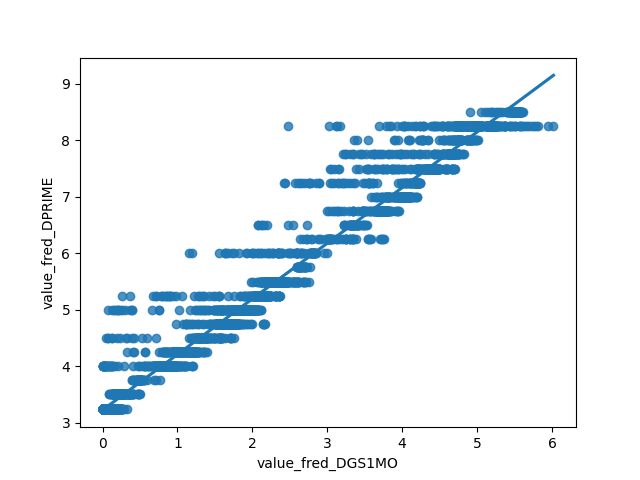
\includegraphics[scale = 0.9]{plots/plot_2026-11-25.png}
\caption{Raw Regression Plot for 2026-11-25}
\end{figure}
\newpage
\subsection{Detrended Regression}
\noindent Regresses the residuals of each series after removing its own linear time trend, so a shared trend can no longer drive the result on its own. A relationship that stays significant here is better evidence of a genuine link between the two series.

\begin{center}
\begin{tabular}{lclc}
\toprule
\textbf{Dep. Variable:}                 & value\_fred\_DPRIME\_detrended & \textbf{  R-squared:         } &     0.981   \\
\textbf{Model:}                         &              OLS               & \textbf{  Adj. R-squared:    } &     0.981   \\
\textbf{Method:}                        &         Least Squares          & \textbf{  F-statistic:       } & 3.339e+05   \\
\textbf{Date:}                          &        Wed, 25 Nov 2026        & \textbf{  Prob (F-statistic):} &     0.00    \\
\textbf{Time:}                          &            20:47:07            & \textbf{  Log-Likelihood:    } &   -85.975   \\
\textbf{No. Observations:}              &               6329             & \textbf{  AIC:               } &     176.0   \\
\textbf{Df Residuals:}                  &               6327             & \textbf{  BIC:               } &     189.5   \\
\textbf{Df Model:}                      &                  1             & \textbf{                     } &             \\
\textbf{Covariance Type:}               &           nonrobust            & \textbf{                     } &             \\
\bottomrule
\end{tabular}
\begin{tabular}{lcccccc}
                                        & \textbf{coef} & \textbf{std err} & \textbf{t} & \textbf{P$> |$t$|$} & \textbf{[0.025} & \textbf{0.975]}  \\
\midrule
\textbf{const}                          &    3.095e-13  &        0.003     &     1e-10  &         1.000        &       -0.006    &        0.006     \\
\textbf{value\_fred\_DGS1MO\_detrended} &       0.9895  &        0.002     &   577.880  &         0.000        &        0.986    &        0.993     \\
\bottomrule
\end{tabular}
\begin{tabular}{lclc}
\textbf{Omnibus:}       & 4451.235 & \textbf{  Durbin-Watson:     } &     0.082  \\
\textbf{Prob(Omnibus):} &   0.000  & \textbf{  Jarque-Bera (JB):  } & 75631.527  \\
\textbf{Skew:}          &   3.216  & \textbf{  Prob(JB):          } &      0.00  \\
\textbf{Kurtosis:}      &  18.666  & \textbf{  Cond. No.          } &      1.80  \\
\bottomrule
\end{tabular}
%\caption{OLS Regression Results}
\end{center}

Notes: \newline
 [1] Standard Errors assume that the covariance matrix of the errors is correctly specified.

\begin{figure}
\centering
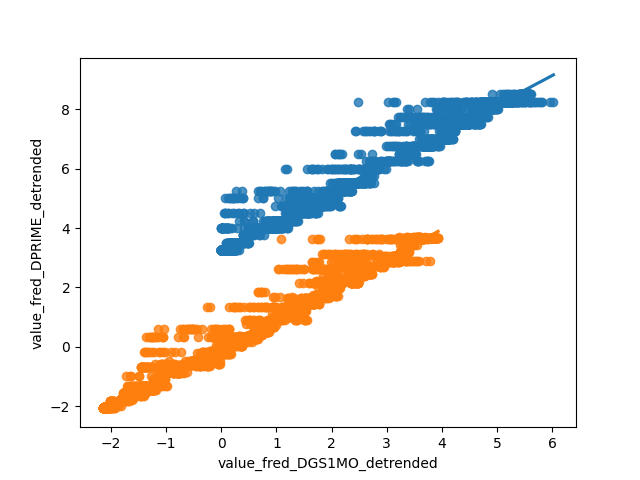
\includegraphics[scale = 0.9]{plots/plot_2026-11-25_detrended.png}
\caption{Detrended Regression Plot for 2026-11-25}
\end{figure}
\newpage
